% Options for packages loaded elsewhere
\PassOptionsToPackage{unicode}{hyperref}
\PassOptionsToPackage{hyphens}{url}
%
\documentclass[
  11pt,
]{article}
\usepackage{amsmath,amssymb}
\usepackage{iftex}
\ifPDFTeX
  \usepackage[T1]{fontenc}
  \usepackage[utf8]{inputenc}
  \usepackage{textcomp} % provide euro and other symbols
\else % if luatex or xetex
  \usepackage{unicode-math} % this also loads fontspec
  \defaultfontfeatures{Scale=MatchLowercase}
  \defaultfontfeatures[\rmfamily]{Ligatures=TeX,Scale=1}
\fi
\usepackage{lmodern}
\ifPDFTeX\else
  % xetex/luatex font selection
\fi
% Use upquote if available, for straight quotes in verbatim environments
\IfFileExists{upquote.sty}{\usepackage{upquote}}{}
\IfFileExists{microtype.sty}{% use microtype if available
  \usepackage[]{microtype}
  \UseMicrotypeSet[protrusion]{basicmath} % disable protrusion for tt fonts
}{}
\makeatletter
\@ifundefined{KOMAClassName}{% if non-KOMA class
  \IfFileExists{parskip.sty}{%
    \usepackage{parskip}
  }{% else
    \setlength{\parindent}{0pt}
    \setlength{\parskip}{6pt plus 2pt minus 1pt}}
}{% if KOMA class
  \KOMAoptions{parskip=half}}
\makeatother
\usepackage{xcolor}
\usepackage[margin=0.5in]{geometry}
\usepackage{longtable,booktabs,array}
\usepackage{calc} % for calculating minipage widths
% Correct order of tables after \paragraph or \subparagraph
\usepackage{etoolbox}
\makeatletter
\patchcmd\longtable{\par}{\if@noskipsec\mbox{}\fi\par}{}{}
\makeatother
% Allow footnotes in longtable head/foot
\IfFileExists{footnotehyper.sty}{\usepackage{footnotehyper}}{\usepackage{footnote}}
\makesavenoteenv{longtable}
\usepackage{graphicx}
\makeatletter
\def\maxwidth{\ifdim\Gin@nat@width>\linewidth\linewidth\else\Gin@nat@width\fi}
\def\maxheight{\ifdim\Gin@nat@height>\textheight\textheight\else\Gin@nat@height\fi}
\makeatother
% Scale images if necessary, so that they will not overflow the page
% margins by default, and it is still possible to overwrite the defaults
% using explicit options in \includegraphics[width, height, ...]{}
\setkeys{Gin}{width=\maxwidth,height=\maxheight,keepaspectratio}
% Set default figure placement to htbp
\makeatletter
\def\fps@figure{htbp}
\makeatother
\setlength{\emergencystretch}{3em} % prevent overfull lines
\providecommand{\tightlist}{%
  \setlength{\itemsep}{0pt}\setlength{\parskip}{0pt}}
\setcounter{secnumdepth}{-\maxdimen} % remove section numbering
% definitions for citeproc citations
\NewDocumentCommand\citeproctext{}{}
\NewDocumentCommand\citeproc{mm}{%
  \begingroup\def\citeproctext{#2}\cite{#1}\endgroup}
\makeatletter
 % allow citations to break across lines
 \let\@cite@ofmt\@firstofone
 % avoid brackets around text for \cite:
 \def\@biblabel#1{}
 \def\@cite#1#2{{#1\if@tempswa , #2\fi}}
\makeatother
\newlength{\cslhangindent}
\setlength{\cslhangindent}{1.5em}
\newlength{\csllabelwidth}
\setlength{\csllabelwidth}{3em}
\newenvironment{CSLReferences}[2] % #1 hanging-indent, #2 entry-spacing
 {\begin{list}{}{%
  \setlength{\itemindent}{0pt}
  \setlength{\leftmargin}{0pt}
  \setlength{\parsep}{0pt}
  % turn on hanging indent if param 1 is 1
  \ifodd #1
   \setlength{\leftmargin}{\cslhangindent}
   \setlength{\itemindent}{-1\cslhangindent}
  \fi
  % set entry spacing
  \setlength{\itemsep}{#2\baselineskip}}}
 {\end{list}}
\usepackage{calc}
\newcommand{\CSLBlock}[1]{\hfill\break#1\hfill\break}
\newcommand{\CSLLeftMargin}[1]{\parbox[t]{\csllabelwidth}{\strut#1\strut}}
\newcommand{\CSLRightInline}[1]{\parbox[t]{\linewidth - \csllabelwidth}{\strut#1\strut}}
\newcommand{\CSLIndent}[1]{\hspace{\cslhangindent}#1}
\usepackage{hyperref}
\usepackage{array}
\usepackage{caption}
\usepackage{graphicx}
\usepackage{multirow}
\usepackage{hhline}
\usepackage{calc}
\usepackage{tabularx}
\usepackage[para,online,flushleft]{threeparttable}
\DeclareMathOperator{\logit}{logit}
\DeclareMathOperator{\var}{var}
\usepackage{float}
\ifLuaTeX
  \usepackage{selnolig}  % disable illegal ligatures
\fi
\IfFileExists{bookmark.sty}{\usepackage{bookmark}}{\usepackage{hyperref}}
\IfFileExists{xurl.sty}{\usepackage{xurl}}{} % add URL line breaks if available
\urlstyle{same}
\hypersetup{
  pdftitle={Analysis of Health Survey for England (HSE) 2019},
  pdfauthor={Candidate Numbers Here},
  hidelinks,
  pdfcreator={LaTeX via pandoc}}

\title{Analysis of Health Survey for England (HSE) 2019}
\author{Candidate Numbers Here}
\date{March 13, 2024}

\begin{document}
\maketitle
\begin{abstract}
This report provides an analysis of data related to health, age,
socio-economic factors and lifestyle habits in adults (from the age of
16) from the population in England, derived from the Health Survey for
England 2019.
\end{abstract}

\pagenumbering{gobble}

\newpage

\subsection{Summary (Non-Technical)}\label{summary-non-technical}

\subsection{Introduction}\label{introduction}

In the UK, smoking, ``vaping'' and alcohol consumption are widespread
habits among adults, particularly younger adults. In fact, it is
estimated that around 14.1\% of UK adults identified as cigarette
smokers (\citeproc{ref-1ONS}{ONS 2019a}), and a similar study found that
there were 7,565 deaths attributed to alcohol-specific causes in 2019
(\citeproc{ref-2ONS}{ONS 2019b}). Thus, it is crucial to be aware of the
predictors and consequences of these habits, which is the motivation for
this analysis. We conducted this analysis on a subset containing 8,204
adults living in England (ages 16+), who were interviewed in their homes
about their demographics and their smoking and drinking habits as part
of the Health Survey for England (HSE) 2019. 4,947 of these participants
who consented to an at-home nurse visit had vitals such as blood
pressure, weight and height measured. We investigated which features of
a participant are associated with smoking habits, and which habits are
associated with high blood pressure. The mechanisms which drive
lifestyle habits are part of a complex and ever-changing field in
behavioural psychology. What is known, however, is that such habits are
driven by cues and cravings (ask Cam for the citation). The HSE 2019
captures demographic and socioeconomic characteristics that have the
potential to make such cues more visible and cravings harder to resist.
For example, living in a region where smoking is more prevalent, like
ones with higher deprivation {[}citation needed{]}, or not having a
husband/wife for an accountability partner to help you quit or resist
these habits. In this report, we will use weighting variables to
estimate prevalence of cigarette, e-cig, and alcohol users in our
population, and compare it with the larger population of adults in
England. We will then attempt to identify associations with a
participants current smoking status, explore whether predictive
modelling can be used to identify smokers with a high accuracy, and
investigate which lifestyle habits are associated with increased values
of systolic blood pressure. \emph{This will be crucial in enabling
healthcare providers to implement preventative care for people at risk
of developing hypertension.}

\subsection{Exploratory Analysis}\label{exploratory-analysis}

The full HSE 2019 cross-sectional data set contains 10,299 observations
across thousands of variables {[}cite the dataset here{]}, but we only
studied patients over the age of 16 among key variables. Our subset
includes 8,204 participants and 19 variables, which are grouped into
five categories and described in Table ??.

\textbf{Table ??}

We found 36 pairs of observations with exactly equal variables
(excluding ID variables and lab measurements), but we did not remove
these from our analysis because the supporting documentation doesn't
state a protocol for repeated visits. We assumed these were genuine
observations from different participants and thus included them in our
dataset. However, there were 3 pairs of observations that had duplicate
lab variables also. We believed that these were true duplicates and
removed one observation from each of the three pairs resulting in a
dataset of 8201 observations.

All variables are coded as numeric in our dataset, so we recoded all
factor variables accordingly. Some of the variables used for analysis
were dichotomised by us for easier interpretation. We coded a binary
variable indicating current smoking status, which will serve as our
\emph{primary} outcome variable. Also, we dichotomised urbanity into two
levels being `Rural' and `Urban', and finally marital status was
dichotomised into `Married' and `Not Married'. We group respondents into
`Higher Education', `Further Education', `A-Level equiv.', `GCSE
equiv.', `No qualification' and `Foreign/other'.

The number of missing observations for each are shown in Table
\ref{tab:output-na-table}:

\begin{longtable}[]{@{}lrl@{}}
\caption{Missing values in the training
dataset\label{tab:output-na-table}}\tabularnewline
\toprule\noalign{}
Variable & Missing Values & \% Missing \\
\midrule\noalign{}
\endfirsthead
\toprule\noalign{}
Variable & Missing Values & \% Missing \\
\midrule\noalign{}
\endhead
\bottomrule\noalign{}
\endlastfoot
omsysval & 4036 & 61.5\% \\
BMIVal & 1519 & 23.2\% \\
dnoft\_19 & 1496 & 22.8\% \\
cigdyal\_19 & 57 & 0.869\% \\
cigsta3\_19 & 56 & 0.854\% \\
NDPNow\_19 & 53 & 0.808\% \\
d7many3\_19 & 52 & 0.793\% \\
drinkYN\_19 & 51 & 0.777\% \\
topqual2 & 46 & 0.701\% \\
origin2 & 29 & 0.442\% \\
marstatD & 1 & 0.0152\% \\
\end{longtable}

There is significant missingness in the lab values, which can be
explained by the fact additional consent was needed from the participant
to allow a nurse visit. One variable with a substantial amount of data
missing was the frequency of drinking in the last 12 months, which due
to the retrospective and sensitive nature of the question could be
explained by either recall bias or a participant's refusal to answer.
Education level, marital status and ethnicity are the only demographic
variables with any missing entries, with 46 observations (0.701\% of the
data) missing at least one of the three. These are not necessary for
identifiability and as they are sensitive, we do not expect every
participant to answer these questions. Therefore, we did not remove
these observations.

We analysed the two lab measurement variables in Figure
\ref{fig:output-distribution-plots}, finding potential outliers to be
present in both. There were many outliers for BMI, which we note used
self-estimated weight from the participant in the calculation when it
exceeded 130kg. Additionally, weight measurements were taken in
inconsistent environments such as on different flooring in the
participants' homes which has been shown in previous research to impact
measurements accuracy {[}citation needed{]}. We believed this could have
explained the extremely high BMI values such as \emph{LIST EXAMPLES},
and so coded them as missing in the analysis dataset.

The readings for systolic blood pressure were collected by taking an
average of three readings, each five minutes apart, performed by a
trained nurse who had to declare each reading to be valid. For this
reason, it seemed highly unlikely that these readings were mistakes, and
so we included them in our analysis. We did, however, note that values
of systolic blood pressure that were this consistently high
(\textgreater140mmHg) were indicators for hypertensive crisis, and so a
part of our population may have serious underlying health conditions
that could affect the generalisability of our findings {[}citation
needed{]}.

\begin{figure}[H]
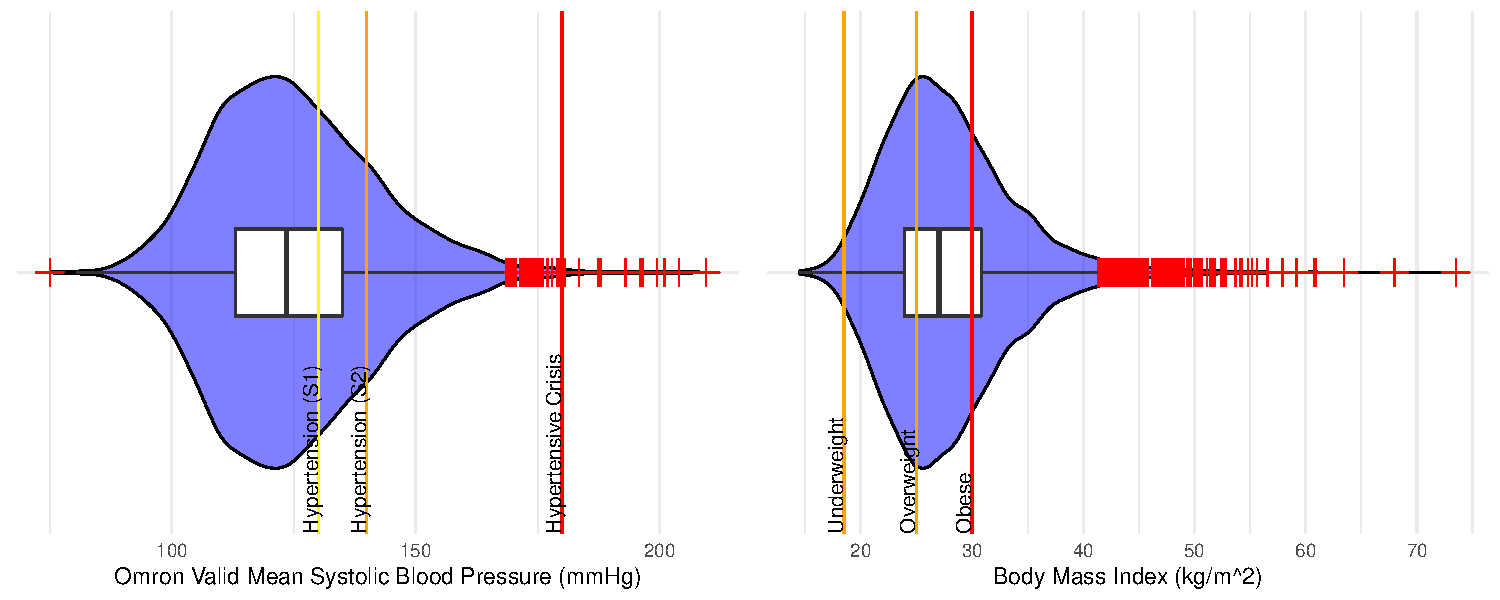
\includegraphics{Coursework_files/figure-latex/output-distribution-plots-1} \caption{Distribution of BMI and Mean Systolic Blood Pressure}\label{fig:output-distribution-plots}
\end{figure}

\subsection{Methology}\label{methology}

\subsubsection{What is the prevelance of drinking, smoking and E-cig
usage?}\label{what-is-the-prevelance-of-drinking-smoking-and-e-cig-usage}

To calculate the prevalence of each habit we assumed each of the \(n\)
observations, \(x_1,…,x_n\) , to be independent, identically distributed
(iid) random variables (RVs) where
\(x_i \sim Bern(p)\, \forall i=1,…,n\) and \(p\) denotes the probability
of an observation having the relevant habit. We use the household
weights to calculate a weighted Maximum Likelihood Estimate (MLE) of
\(p\). That is, letting \(w_i\) denote the weight of the \(i^{th}\)
observation, we altered the standard likelihood function of a Bernoulli
distribution as below:
\[L(p|\textbf{x}) = \prod_{i = 1}^{n} (p^{x_i}(1-p)^{1-x_i})^{w_i}\]
From this, we calculated our weighted MLE as
\(\widehat{p} = \frac{\sum_{i=1}^{n} x_iw_i}{\sum_{i=1}^{n} w_i}\). It
can also be shown that this MLE has variance given by
\(\mathop{\mathrm{var}}(\widehat{p})=\frac{p(1-p)}{\sum_{i=1}^{n}w_i}\),
which we estimated using \(\widehat{p}\). We used large sample
properties of the MLE to get a normal approximation and estimated 95\%
confidence intervals for each habit, which are shown in Table
\ref{tab:output-estimates-table}.

\begin{longtable}[]{@{}lll@{}}
\caption{Estimates and 95\% Confidence Intervals for \% of
Population\label{tab:output-estimates-table}}\tabularnewline
\toprule\noalign{}
Habit & Estimate & C.I. \\
\midrule\noalign{}
\endfirsthead
\toprule\noalign{}
Habit & Estimate & C.I. \\
\midrule\noalign{}
\endhead
\bottomrule\noalign{}
\endlastfoot
Drinking & 80.4\% & (79.5\%, 81.2\%) \\
Smoking & 16.5\% & (15.7\%, 17.3\%) \\
Smoking E-cigarettes & 4.28\% & (3.84\%, 4.72\%) \\
\end{longtable}

We found that the usage of e-cigarette usage among adults is relatively
low, making it challenging to dissect any significant trends within the
data. \emph{Maybe a wee bit more here}

Next, we worked to uncover factors that have possible associations with
smoking prevalence. We started with the demographic factors of age and
gender, plotting the smoking prevalence across combinations of these
groups to identify any patterns. Figure \ref{fig:output-prevelance-plot}
suggests a negative correlation between age and the proportion of
current cigarette smokers, across both genders. Interestingly, the
proportion of males who quit smoking in later-life was much greater than
that of females (75yrs+; M: 50\%, F: 31\%), which could be attributed to
men being at a higher risk of smoking-related diseases {[}citation
needed{]}.

\begin{figure}[H]
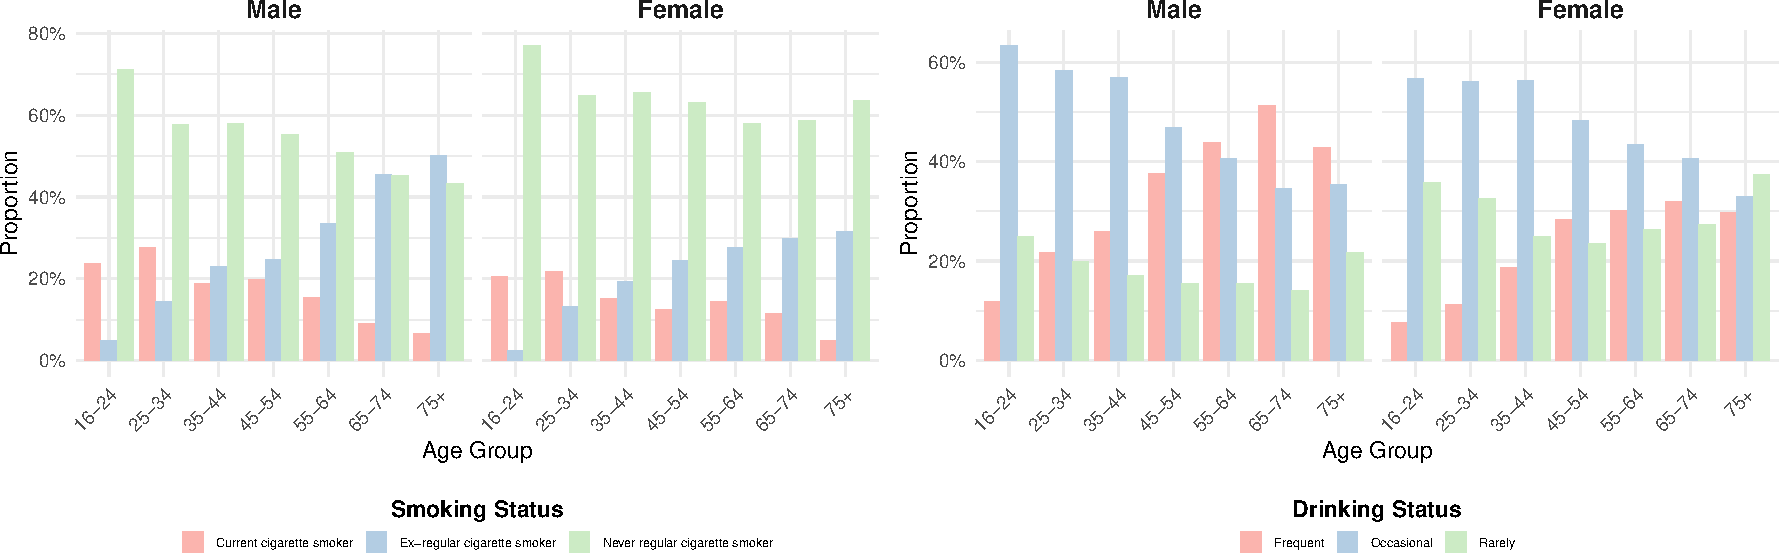
\includegraphics{Coursework_files/figure-latex/output-smoking-drinking-age-plot-1} \caption{Smoking and drinking status proportions by age group and gender}\label{fig:output-smoking-drinking-age-plot}
\end{figure}

\begin{figure}[H]
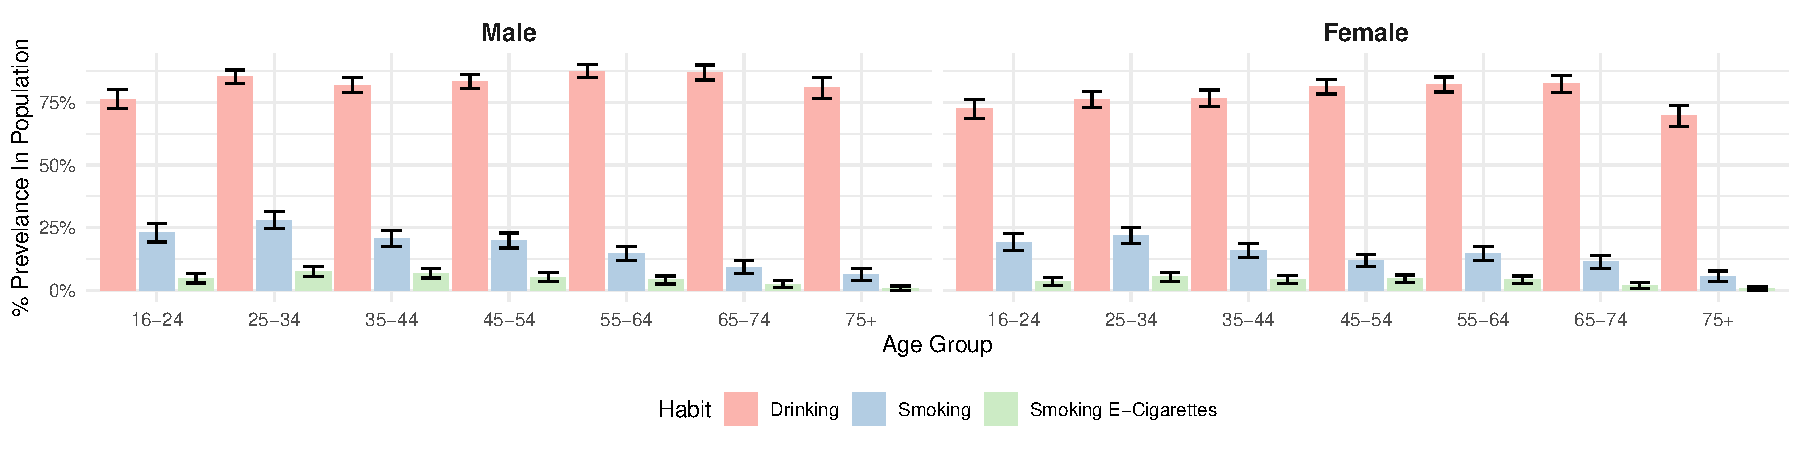
\includegraphics{Coursework_files/figure-latex/output-prevelance-plot-1} \caption{Estimation of the prevelance of smokers by deprivation}\label{fig:output-prevelance-plot}
\end{figure}

\emph{Additionally, males demonstrate a higher prevalence of drinking
across nearly all demographic categories in comparison to females.}
\emph{We can clearly see that smoking prevalence increases with our
deprivation variable, meaning that smokers tend to be from lower levels
of deprivation. This correlation may be caused by the hefty tobacco
duties the UK impose on its' residents (\citeproc{ref-GovUK}{GOV.UK
2014}). Less deprived individuals they can take-up more unnecessary,
expensive habits, with smoking being one of the main candidates.}

\subsubsection{How is smoking associated with socioeconomic factors and
age?}\label{how-is-smoking-associated-with-socioeconomic-factors-and-age}

We reserved 80\% of our data to train the model, and used the remaining
20\% to test the model, which was made possible due to the large size of
our dataset. The training set contained 6561 observations and the test
set contained 1640. \emph{Table Z summarises the key variables between
the test and train dataset to illustrate that both are representative of
the whole dataset.} This reduced the risk of overfitting and allowed us
to test the predictive power of each model we proposed.

To develop a predictive model for identifying smokers, we used the
binary variable for current smoking status as a response, with various
socioeconomic and demographic factors as predictors. These were selected
based on the associations suggested by our prior analysis.

In the dataset, there were two variables that categorised age. They
differed only in the size of the bands used, with one using 10-year
bands and one using 5-year bands. After comparing identical models that
used one or the other, we found that modelling with smaller bands
improved the effectiveness of the model.

Under the assumption that ages were approximately uniformly distributed
within their respective age bands, we also defined the estimated age of
the \(i^{th}\) observation as the midpoint of their respective 5-year
age bracket (taking the estimation of the 90+ category as 92.5), denoted
\(a_i\). We found that age may represent a somewhat quadratic effect on
the probability of smoking, leading us to include a \(a_i^2\) term in
our model. A comparison of these models are summarised in Table
\ref{tab:output-model-selection-table}.

\begin{longtable}[]{@{}
  >{\raggedright\arraybackslash}p{(\columnwidth - 10\tabcolsep) * \real{0.5940}}
  >{\raggedleft\arraybackslash}p{(\columnwidth - 10\tabcolsep) * \real{0.0752}}
  >{\raggedleft\arraybackslash}p{(\columnwidth - 10\tabcolsep) * \real{0.0677}}
  >{\raggedleft\arraybackslash}p{(\columnwidth - 10\tabcolsep) * \real{0.0827}}
  >{\raggedleft\arraybackslash}p{(\columnwidth - 10\tabcolsep) * \real{0.0752}}
  >{\raggedleft\arraybackslash}p{(\columnwidth - 10\tabcolsep) * \real{0.1053}}@{}}
\caption{Comparison of selected model
evaluations\label{tab:output-model-selection-table}}\tabularnewline
\toprule\noalign{}
\begin{minipage}[b]{\linewidth}\raggedright
Linear Predictor
\end{minipage} & \begin{minipage}[b]{\linewidth}\raggedleft
Train AIC
\end{minipage} & \begin{minipage}[b]{\linewidth}\raggedleft
Test AUC
\end{minipage} & \begin{minipage}[b]{\linewidth}\raggedleft
Train RMSE
\end{minipage} & \begin{minipage}[b]{\linewidth}\raggedleft
Test RMSE
\end{minipage} & \begin{minipage}[b]{\linewidth}\raggedleft
Test Accuracy
\end{minipage} \\
\midrule\noalign{}
\endfirsthead
\toprule\noalign{}
\begin{minipage}[b]{\linewidth}\raggedright
Linear Predictor
\end{minipage} & \begin{minipage}[b]{\linewidth}\raggedleft
Train AIC
\end{minipage} & \begin{minipage}[b]{\linewidth}\raggedleft
Test AUC
\end{minipage} & \begin{minipage}[b]{\linewidth}\raggedleft
Train RMSE
\end{minipage} & \begin{minipage}[b]{\linewidth}\raggedleft
Test RMSE
\end{minipage} & \begin{minipage}[b]{\linewidth}\raggedleft
Test Accuracy
\end{minipage} \\
\midrule\noalign{}
\endhead
\bottomrule\noalign{}
\endlastfoot
\(\mathop{\mathrm{logit}}(\mu_i) \sim a_i + a_i^2 + m_i + q_i + u_i + o_i + t_i + s_i + q_i:u_i\)
& 4987.5 & 0.759 & 0.342 & 0.324 & 0.861 \\
\(\mathop{\mathrm{logit}}(\mu_i) \sim a_i + a_i^2 + m_i + q_i + u_i + o_i + t_i + s_i\)
& 4987.3 & 0.759 & 0.342 & 0.324 & 0.861 \\
\(\mathop{\mathrm{logit}}(\mu_i) \sim a_i + m_i + q_i + u_i + o_i + t_i + s_i\)
& 5036.4 & 0.740 & 0.343 & 0.327 & 0.861 \\
\(\mathop{\mathrm{logit}}(\mu_i) \sim a_i^{(5)} + m_i + q_i + u_i + o_i + t_i + s_i\)
& 4994.3 & 0.759 & 0.341 & 0.325 & 0.861 \\
\(\mathop{\mathrm{logit}}(\mu_i) \sim a_i^{(10)} + m_i + q_i + u_i + o_i + t_i + s_i\)
& 5005.9 & 0.753 & 0.342 & 0.324 & 0.860 \\
\end{longtable}

We selected the model based on AIC, which enabled us to balance model
complexity and model fit. This model is \emph{change factors}
\[\mathop{\mathrm{logit}}(\mu_i) \sim \beta_0 + \beta_1a + \beta_2a^2 + \beta_3q + \alpha^{m}_j + \alpha^{u}_k + \alpha^{o}_l + \alpha^{t}_m + \alpha^{s}_n + \beta^{*}_kq\]
where \(j \in \{Married,Not\,Married\}\),
\(k \in \{Urban,Not\,Urban\}\), \(l \in \{White,...,Other\}\),
\(n \in \{Male,Female\}\) and
\(m \in \{Further\,Education,...,No\,qualification\}\).

To evaluate the predictive performance of our final model using our test
data, Figure \ref{fig:output-calibration-chart} demonstrates the
predicted probability of each `probability bin' against the mean actual
outcomes. As we can see the calibration curve closely follows the line
\(y = x\), which is indicative of a well-calibrated model. \emph{This
model doesn't predict high values\ldots{}}

\begin{figure}[H]

{\centering 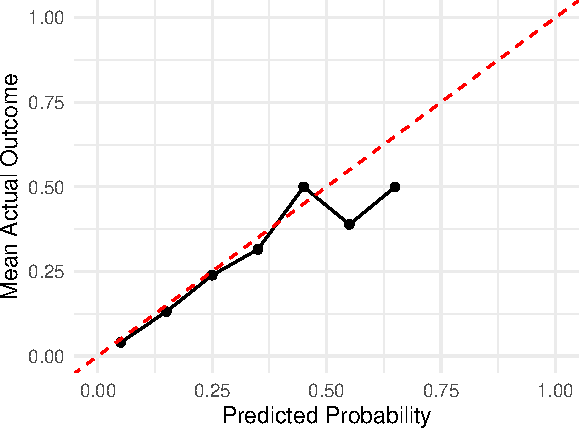
\includegraphics{Coursework_files/figure-latex/output-calibration-chart-1} 

}

\caption{Calibration chart for Binomial model}\label{fig:output-calibration-chart}
\end{figure}

\subsubsection{Which lifestyle habits are associated with systolic blood
pressure?}\label{which-lifestyle-habits-are-associated-with-systolic-blood-pressure}

\begin{figure}[H]
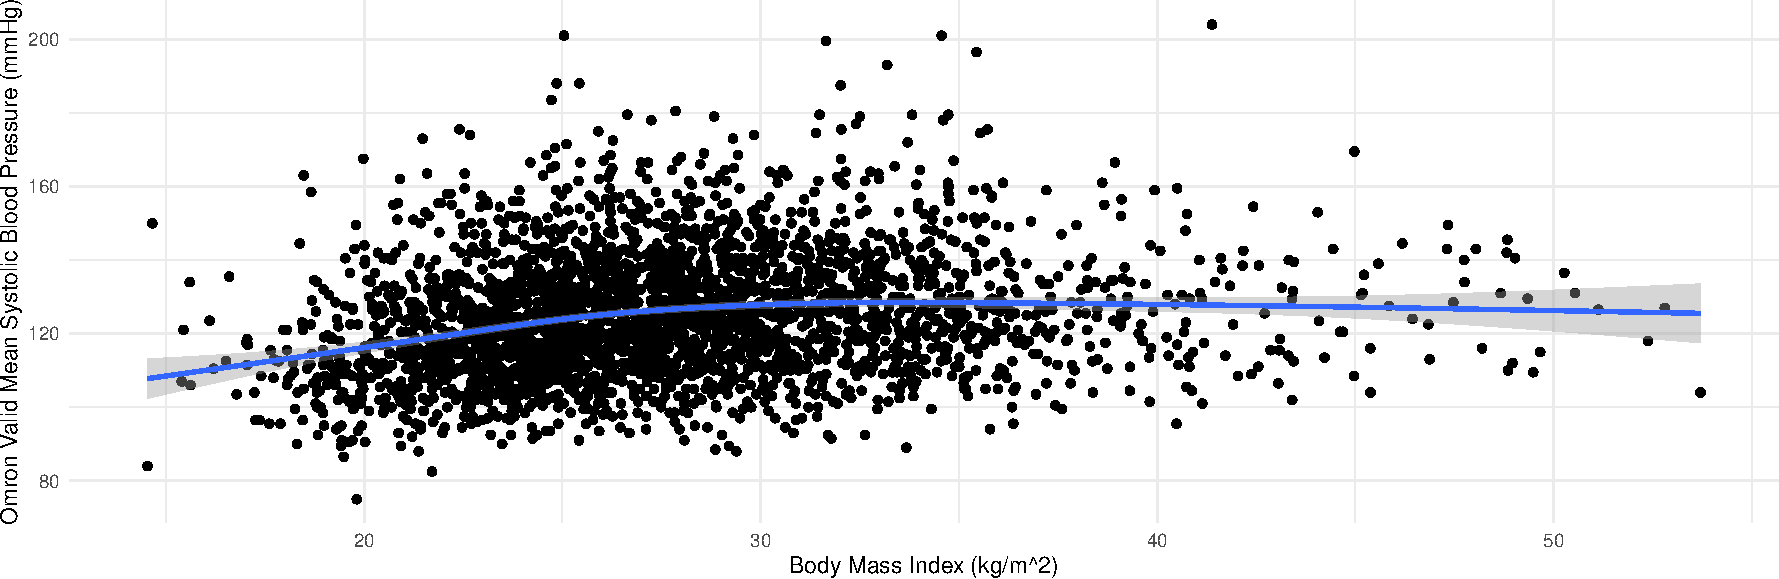
\includegraphics{Coursework_files/figure-latex/output relationship plots-1} \caption{Relationship of BMI and Age with Mean Systolic Blood Pressure}\label{fig:output relationship plots}
\end{figure}

\begin{figure}[H]

{\centering 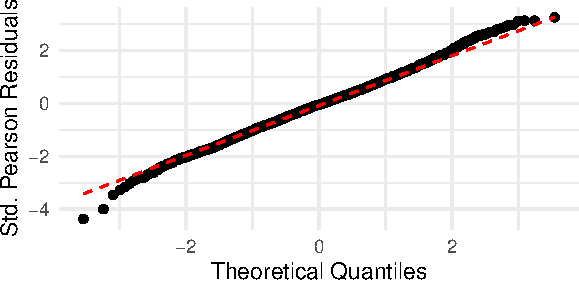
\includegraphics{Coursework_files/figure-latex/output qq plot for q3-1} 

}

\caption{Q-Q plot of Inverse-Normal model residuals}\label{fig:output qq plot for q3}
\end{figure}

\subsection{Results/Conclusion}\label{resultsconclusion}

Our analysis showed that alcohol consumption is extremely common among
UK adults, with approximately 80.4\% being consumers, while smoking and
vaping rates are lower at 16.5\% and 4.3\%, respectively. Older males
show the highest tendencies for alcohol consumption, with `frequent'
drinking the most prevalent among males aged 65-74. Unlike `frequent'
alcohol consumption, the prevalence of smoking decreases with age.
Individuals aged 16-24 appear to be the worst offenders when it comes to
smoking cigarettes, indicating a significant issue within youth culture.
Moreover, we found an interesting relationship between deprivation
levels and smoking and drinking behaviours. Smoking prevalence seemed to
increase as deprivation levels decrease, while alcohol consumption
appeared to do the opposite.

To help us uncover the underlying socio-economic factors that may drive
the prevalence of smoking, we first looked at the most `comparable'
respondent type in our dataset. This `respondent' is a white, single
male who has no qualifications and lives in an urban area. We found that
the probability of our hypothetical respondent being a smoker is
approximately 25\% \emph{Where is this from?} (notably higher than the
population average of 16.5). \emph{Maybe worth talking about confidence
intervals here - is value outside 95\%} The only socio-economic
variables to certainly increase this probability is the deprivation
level our respondent falls under. The rest of the socio-economic
variables we have access to, appear to decrease the likelihood of
smoking. For example, if our respondent is any of the following: Asian,
black, married, or went on to further education, the chances of them
being a smoker is at-least halved.

NatCen Social Research and Health (\citeproc{ref-Main}{2019}) \emph{?}

\newpage

\section*{References}\label{references}
\addcontentsline{toc}{section}{References}

\phantomsection\label{refs}
\begin{CSLReferences}{1}{0}
\bibitem[\citeproctext]{ref-GovUK}
GOV.UK. 2014. {``{Tax on shopping and services}.''}
\url{https://www.gov.uk/tax-on-shopping/alcohol-tobacco}.

\bibitem[\citeproctext]{ref-Main}
NatCen Social Research, Department of Epidemiology, University College
London, and Public Health. 2019. {``{Health Survey for England}.''}
\url{http://doi.org/10.5255/UKDA-SN-8860-1}.

\bibitem[\citeproctext]{ref-1ONS}
ONS. 2019a. {``{Adult smoking habits in the UK: 2019}.''}
\url{https://shorturl.at/qQW27}.

\bibitem[\citeproctext]{ref-2ONS}
---------. 2019b. {``{Alcohol-specific deaths in the UK: registered in
2019}.''} \url{https://shorturl.at/gqxY1}.

\end{CSLReferences}

\end{document}
